% Options for packages loaded elsewhere
\PassOptionsToPackage{unicode}{hyperref}
\PassOptionsToPackage{hyphens}{url}
\PassOptionsToPackage{dvipsnames,svgnames,x11names}{xcolor}
%
\documentclass[
  letterpaper,
  DIV=11,
  numbers=noendperiod]{scrartcl}

\usepackage{amsmath,amssymb}
\usepackage{iftex}
\ifPDFTeX
  \usepackage[T1]{fontenc}
  \usepackage[utf8]{inputenc}
  \usepackage{textcomp} % provide euro and other symbols
\else % if luatex or xetex
  \usepackage{unicode-math}
  \defaultfontfeatures{Scale=MatchLowercase}
  \defaultfontfeatures[\rmfamily]{Ligatures=TeX,Scale=1}
\fi
\usepackage{lmodern}
\ifPDFTeX\else  
    % xetex/luatex font selection
  \setmainfont[]{cochineal}
  \setsansfont[]{Helvetica}
\fi
% Use upquote if available, for straight quotes in verbatim environments
\IfFileExists{upquote.sty}{\usepackage{upquote}}{}
\IfFileExists{microtype.sty}{% use microtype if available
  \usepackage[]{microtype}
  \UseMicrotypeSet[protrusion]{basicmath} % disable protrusion for tt fonts
}{}
\makeatletter
\@ifundefined{KOMAClassName}{% if non-KOMA class
  \IfFileExists{parskip.sty}{%
    \usepackage{parskip}
  }{% else
    \setlength{\parindent}{0pt}
    \setlength{\parskip}{6pt plus 2pt minus 1pt}}
}{% if KOMA class
  \KOMAoptions{parskip=half}}
\makeatother
\usepackage{xcolor}
\usepackage[margin = 1.0in]{geometry}
\setlength{\emergencystretch}{3em} % prevent overfull lines
\setcounter{secnumdepth}{5}
% Make \paragraph and \subparagraph free-standing
\ifx\paragraph\undefined\else
  \let\oldparagraph\paragraph
  \renewcommand{\paragraph}[1]{\oldparagraph{#1}\mbox{}}
\fi
\ifx\subparagraph\undefined\else
  \let\oldsubparagraph\subparagraph
  \renewcommand{\subparagraph}[1]{\oldsubparagraph{#1}\mbox{}}
\fi

\usepackage{color}
\usepackage{fancyvrb}
\newcommand{\VerbBar}{|}
\newcommand{\VERB}{\Verb[commandchars=\\\{\}]}
\DefineVerbatimEnvironment{Highlighting}{Verbatim}{commandchars=\\\{\}}
% Add ',fontsize=\small' for more characters per line
\usepackage{framed}
\definecolor{shadecolor}{RGB}{241,243,245}
\newenvironment{Shaded}{\begin{snugshade}}{\end{snugshade}}
\newcommand{\AlertTok}[1]{\textcolor[rgb]{0.68,0.00,0.00}{#1}}
\newcommand{\AnnotationTok}[1]{\textcolor[rgb]{0.37,0.37,0.37}{#1}}
\newcommand{\AttributeTok}[1]{\textcolor[rgb]{0.40,0.45,0.13}{#1}}
\newcommand{\BaseNTok}[1]{\textcolor[rgb]{0.68,0.00,0.00}{#1}}
\newcommand{\BuiltInTok}[1]{\textcolor[rgb]{0.00,0.23,0.31}{#1}}
\newcommand{\CharTok}[1]{\textcolor[rgb]{0.13,0.47,0.30}{#1}}
\newcommand{\CommentTok}[1]{\textcolor[rgb]{0.37,0.37,0.37}{#1}}
\newcommand{\CommentVarTok}[1]{\textcolor[rgb]{0.37,0.37,0.37}{\textit{#1}}}
\newcommand{\ConstantTok}[1]{\textcolor[rgb]{0.56,0.35,0.01}{#1}}
\newcommand{\ControlFlowTok}[1]{\textcolor[rgb]{0.00,0.23,0.31}{#1}}
\newcommand{\DataTypeTok}[1]{\textcolor[rgb]{0.68,0.00,0.00}{#1}}
\newcommand{\DecValTok}[1]{\textcolor[rgb]{0.68,0.00,0.00}{#1}}
\newcommand{\DocumentationTok}[1]{\textcolor[rgb]{0.37,0.37,0.37}{\textit{#1}}}
\newcommand{\ErrorTok}[1]{\textcolor[rgb]{0.68,0.00,0.00}{#1}}
\newcommand{\ExtensionTok}[1]{\textcolor[rgb]{0.00,0.23,0.31}{#1}}
\newcommand{\FloatTok}[1]{\textcolor[rgb]{0.68,0.00,0.00}{#1}}
\newcommand{\FunctionTok}[1]{\textcolor[rgb]{0.28,0.35,0.67}{#1}}
\newcommand{\ImportTok}[1]{\textcolor[rgb]{0.00,0.46,0.62}{#1}}
\newcommand{\InformationTok}[1]{\textcolor[rgb]{0.37,0.37,0.37}{#1}}
\newcommand{\KeywordTok}[1]{\textcolor[rgb]{0.00,0.23,0.31}{#1}}
\newcommand{\NormalTok}[1]{\textcolor[rgb]{0.00,0.23,0.31}{#1}}
\newcommand{\OperatorTok}[1]{\textcolor[rgb]{0.37,0.37,0.37}{#1}}
\newcommand{\OtherTok}[1]{\textcolor[rgb]{0.00,0.23,0.31}{#1}}
\newcommand{\PreprocessorTok}[1]{\textcolor[rgb]{0.68,0.00,0.00}{#1}}
\newcommand{\RegionMarkerTok}[1]{\textcolor[rgb]{0.00,0.23,0.31}{#1}}
\newcommand{\SpecialCharTok}[1]{\textcolor[rgb]{0.37,0.37,0.37}{#1}}
\newcommand{\SpecialStringTok}[1]{\textcolor[rgb]{0.13,0.47,0.30}{#1}}
\newcommand{\StringTok}[1]{\textcolor[rgb]{0.13,0.47,0.30}{#1}}
\newcommand{\VariableTok}[1]{\textcolor[rgb]{0.07,0.07,0.07}{#1}}
\newcommand{\VerbatimStringTok}[1]{\textcolor[rgb]{0.13,0.47,0.30}{#1}}
\newcommand{\WarningTok}[1]{\textcolor[rgb]{0.37,0.37,0.37}{\textit{#1}}}

\providecommand{\tightlist}{%
  \setlength{\itemsep}{0pt}\setlength{\parskip}{0pt}}\usepackage{longtable,booktabs,array}
\usepackage{calc} % for calculating minipage widths
% Correct order of tables after \paragraph or \subparagraph
\usepackage{etoolbox}
\makeatletter
\patchcmd\longtable{\par}{\if@noskipsec\mbox{}\fi\par}{}{}
\makeatother
% Allow footnotes in longtable head/foot
\IfFileExists{footnotehyper.sty}{\usepackage{footnotehyper}}{\usepackage{footnote}}
\makesavenoteenv{longtable}
\usepackage{graphicx}
\makeatletter
\def\maxwidth{\ifdim\Gin@nat@width>\linewidth\linewidth\else\Gin@nat@width\fi}
\def\maxheight{\ifdim\Gin@nat@height>\textheight\textheight\else\Gin@nat@height\fi}
\makeatother
% Scale images if necessary, so that they will not overflow the page
% margins by default, and it is still possible to overwrite the defaults
% using explicit options in \includegraphics[width, height, ...]{}
\setkeys{Gin}{width=\maxwidth,height=\maxheight,keepaspectratio}
% Set default figure placement to htbp
\makeatletter
\def\fps@figure{htbp}
\makeatother
\newlength{\cslhangindent}
\setlength{\cslhangindent}{1.5em}
\newlength{\csllabelwidth}
\setlength{\csllabelwidth}{3em}
\newlength{\cslentryspacingunit} % times entry-spacing
\setlength{\cslentryspacingunit}{\parskip}
\newenvironment{CSLReferences}[2] % #1 hanging-ident, #2 entry spacing
 {% don't indent paragraphs
  \setlength{\parindent}{0pt}
  % turn on hanging indent if param 1 is 1
  \ifodd #1
  \let\oldpar\par
  \def\par{\hangindent=\cslhangindent\oldpar}
  \fi
  % set entry spacing
  \setlength{\parskip}{#2\cslentryspacingunit}
 }%
 {}
\usepackage{calc}
\newcommand{\CSLBlock}[1]{#1\hfill\break}
\newcommand{\CSLLeftMargin}[1]{\parbox[t]{\csllabelwidth}{#1}}
\newcommand{\CSLRightInline}[1]{\parbox[t]{\linewidth - \csllabelwidth}{#1}\break}
\newcommand{\CSLIndent}[1]{\hspace{\cslhangindent}#1}

\usepackage{fontspec}
\usepackage{multirow}
\usepackage{multicol}
\usepackage{colortbl}
\usepackage{hhline}
\newlength\Oldarrayrulewidth
\newlength\Oldtabcolsep
\usepackage{longtable}
\usepackage{array}
\usepackage{hyperref}
\usepackage{float}
\usepackage{wrapfig}
\KOMAoption{captions}{tableheading}
\usepackage{booktabs} \usepackage{setspace} \doublespacing \usepackage[left]{lineno} \linenumbers
\makeatletter
\makeatother
\makeatletter
\makeatother
\makeatletter
\@ifpackageloaded{caption}{}{\usepackage{caption}}
\AtBeginDocument{%
\ifdefined\contentsname
  \renewcommand*\contentsname{Table of contents}
\else
  \newcommand\contentsname{Table of contents}
\fi
\ifdefined\listfigurename
  \renewcommand*\listfigurename{List of Figures}
\else
  \newcommand\listfigurename{List of Figures}
\fi
\ifdefined\listtablename
  \renewcommand*\listtablename{List of Tables}
\else
  \newcommand\listtablename{List of Tables}
\fi
\ifdefined\figurename
  \renewcommand*\figurename{Figure}
\else
  \newcommand\figurename{Figure}
\fi
\ifdefined\tablename
  \renewcommand*\tablename{Table}
\else
  \newcommand\tablename{Table}
\fi
}
\@ifpackageloaded{float}{}{\usepackage{float}}
\floatstyle{ruled}
\@ifundefined{c@chapter}{\newfloat{codelisting}{h}{lop}}{\newfloat{codelisting}{h}{lop}[chapter]}
\floatname{codelisting}{Listing}
\newcommand*\listoflistings{\listof{codelisting}{List of Listings}}
\makeatother
\makeatletter
\@ifpackageloaded{caption}{}{\usepackage{caption}}
\@ifpackageloaded{subcaption}{}{\usepackage{subcaption}}
\makeatother
\makeatletter
\@ifpackageloaded{tcolorbox}{}{\usepackage[skins,breakable]{tcolorbox}}
\makeatother
\makeatletter
\@ifundefined{shadecolor}{\definecolor{shadecolor}{rgb}{.97, .97, .97}}
\makeatother
\makeatletter
\makeatother
\makeatletter
\makeatother
\ifLuaTeX
  \usepackage{selnolig}  % disable illegal ligatures
\fi
\IfFileExists{bookmark.sty}{\usepackage{bookmark}}{\usepackage{hyperref}}
\IfFileExists{xurl.sty}{\usepackage{xurl}}{} % add URL line breaks if available
\urlstyle{same} % disable monospaced font for URLs
\hypersetup{
  colorlinks=true,
  linkcolor={blue},
  filecolor={Maroon},
  citecolor={Blue},
  urlcolor={Blue},
  pdfcreator={LaTeX via pandoc}}

\author{}
\date{}

\begin{document}
\ifdefined\Shaded\renewenvironment{Shaded}{\begin{tcolorbox}[sharp corners, frame hidden, interior hidden, borderline west={3pt}{0pt}{shadecolor}, boxrule=0pt, enhanced, breakable]}{\end{tcolorbox}}\fi

\date{\today}
\title{\textbf{Replication materials are great but software versioning still poses a problem for open science}}

Taylor J.
Wright\thanks{Brock University, \href{mailto:twright3@brocku.ca}{twright3@brocku.ca}}
\textbackslash and

\author{Bruno Rodrigues \thanks{Ministry of Higher Education and Research, Luxembourg}
}

\maketitle

\newpage

\hypertarget{introduction}{%
\section{Introduction}\label{introduction}}

In recent years, the `'replication crisis'' in the social sciences has
become mainstream, even featured in the popular press. Concerns over how
well studies hold up to replication in other settings has lead to large
scale initiatives to document how trustworthy the existing stock of
evidence is (cite Camerer and Nosek). While the replicability of studies
in important, there has been a tandem movement discussing how
reproducible research results are. There are various definitions, but
for broadly speaking replication is in some sense re-testing a
hypothesis while changing an element of previous research (e.g.~the
sample, or the estimating equation) whereas reproducibility is following
a study's protocol exactly and obtaining the results presented in the
study (insert a citation with some definitions here, perhaps Lars' blog
or Michael Clemens JES paper?). In our view, reproducibility is an
insufficient but necessary condition for replication---that is, it does
not make sense to spend resources on replciation if research is not
reproducible.

These concerns about the reproducibility and replicability of social
science research have prompted a push for journals to require the
publication of research materials that accompany academic research (see,
for example, the 2014 Joint Editors Transparency Statement which was
signed by editors of 27 leading political science journals:
\url{https://www.dartstatement.org/2014-journal-editors-statement-jets}).
Specifically, the provision of underlying data and scripts used for data
preparation and analysis. However, even if these materials are provided
(and even when in place these policies do not have perfect compliance
(Philip (2010), Stockemer, Koehler, and Lentz (2018))), the regular
software updates and new version releases can result in the replication
materials failing to faithfully reproduce the authors' results or even
run at all (Simonsohn (2021) presents several examples of \texttt{R}
changes that could break scripts).

In this paper we ppresent a case study of an article published in
Journal of Politics in January 2022 titled, ``Multiracial Identity and
Political Preferences'`, Davenport, Franco, and Iyengar (2022), that
details that replication challenges arising from changes in the
statistical software \texttt{R}. We were unable to reproduce the
authors' results using either the current version of \texttt{R}, or the
version that the authors indicate they used. The lack of reproducibility
arose due to a change in the defaults used by base \texttt{R} when
generating random numbers starting in version 3.6.0.

We contribute to the existing literature\ldots{}

The rest of the article proceeds as follows: Section 2 walks through the
reproducibility issues in Davenport, Franco, and Iyengar (2022); Section
3 discusses currently available tools and best practices (e.g.~Docker
and \texttt{R} packages such as \texttt{renv}, \texttt{groundhog}) for
ensuring that replication materials continue to faithfully reproduce
research results, despite post-publication changes in the tools used;
and Section 4 concludes.

\newpage

\hypertarget{reproduction}{%
\section{Reproduction}\label{reproduction}}

\hypertarget{illustrating-the-issue-with-software-versioning}{%
\subsection{Illustrating the issue with software
versioning}\label{illustrating-the-issue-with-software-versioning}}

A key thing here is that I don't think we want to be too hostile
sounding towards these authors, they had readme files and
reproducibility materials available. It's just that manual entry
human-error hobgoblins got them with the R versioning.

\begin{itemize}
\tightlist
\item
  Brief discussion of authors' paper and context
\item
  The results of their code using stated software version in
  documentation (just screenshot right now)
\end{itemize}

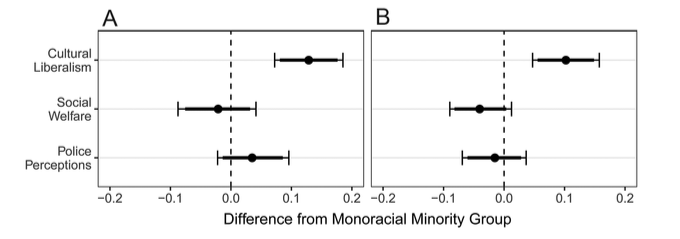
\includegraphics[width=1\textwidth,height=\textheight]{./figures/figure1_screenshot.png}

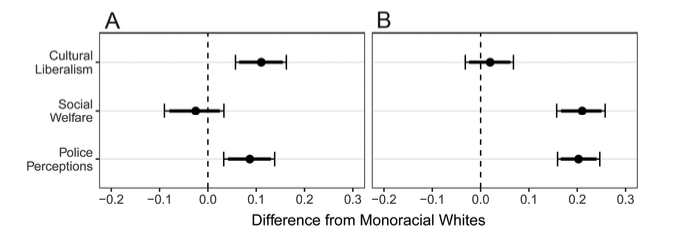
\includegraphics[width=1\textwidth,height=\textheight]{./figures/figure2_screenshot.png}

\begin{itemize}
\tightlist
\item
  The results of their code using later software version (post 3.6.0)
\end{itemize}

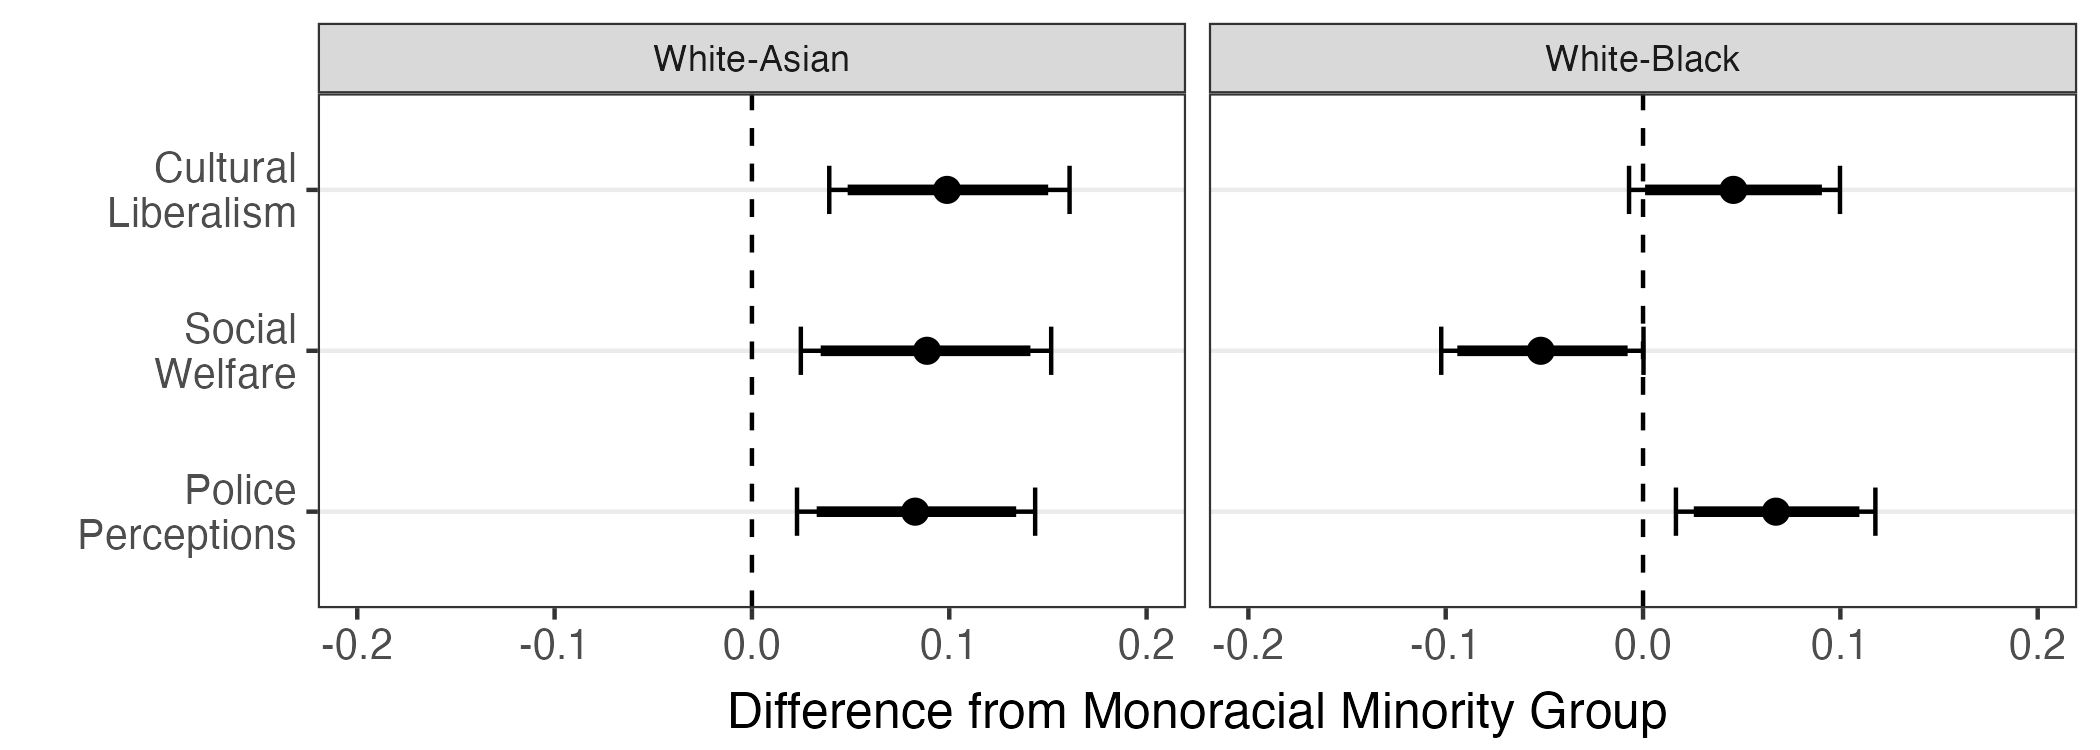
\includegraphics[width=1\textwidth,height=\textheight]{./figures/figure1_postchange.png}

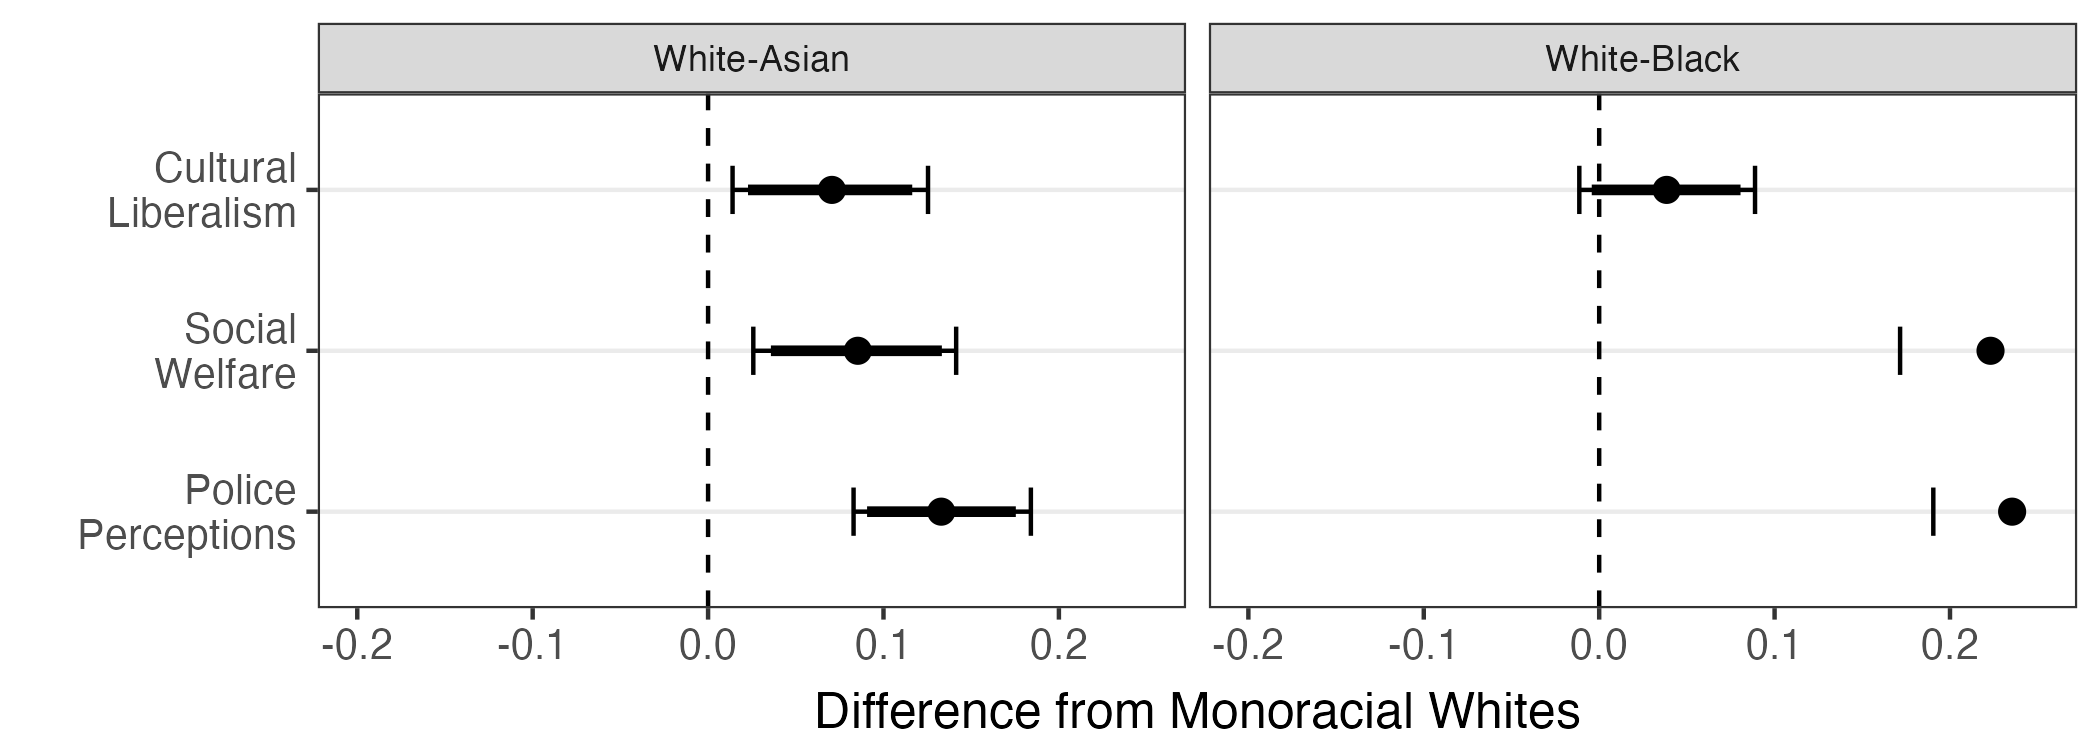
\includegraphics[width=1\textwidth,height=\textheight]{./figures/figure2_postchange.png}

\begin{itemize}
\tightlist
\item
  Results of their code using earlier software version (pre 3.6.0)
\end{itemize}

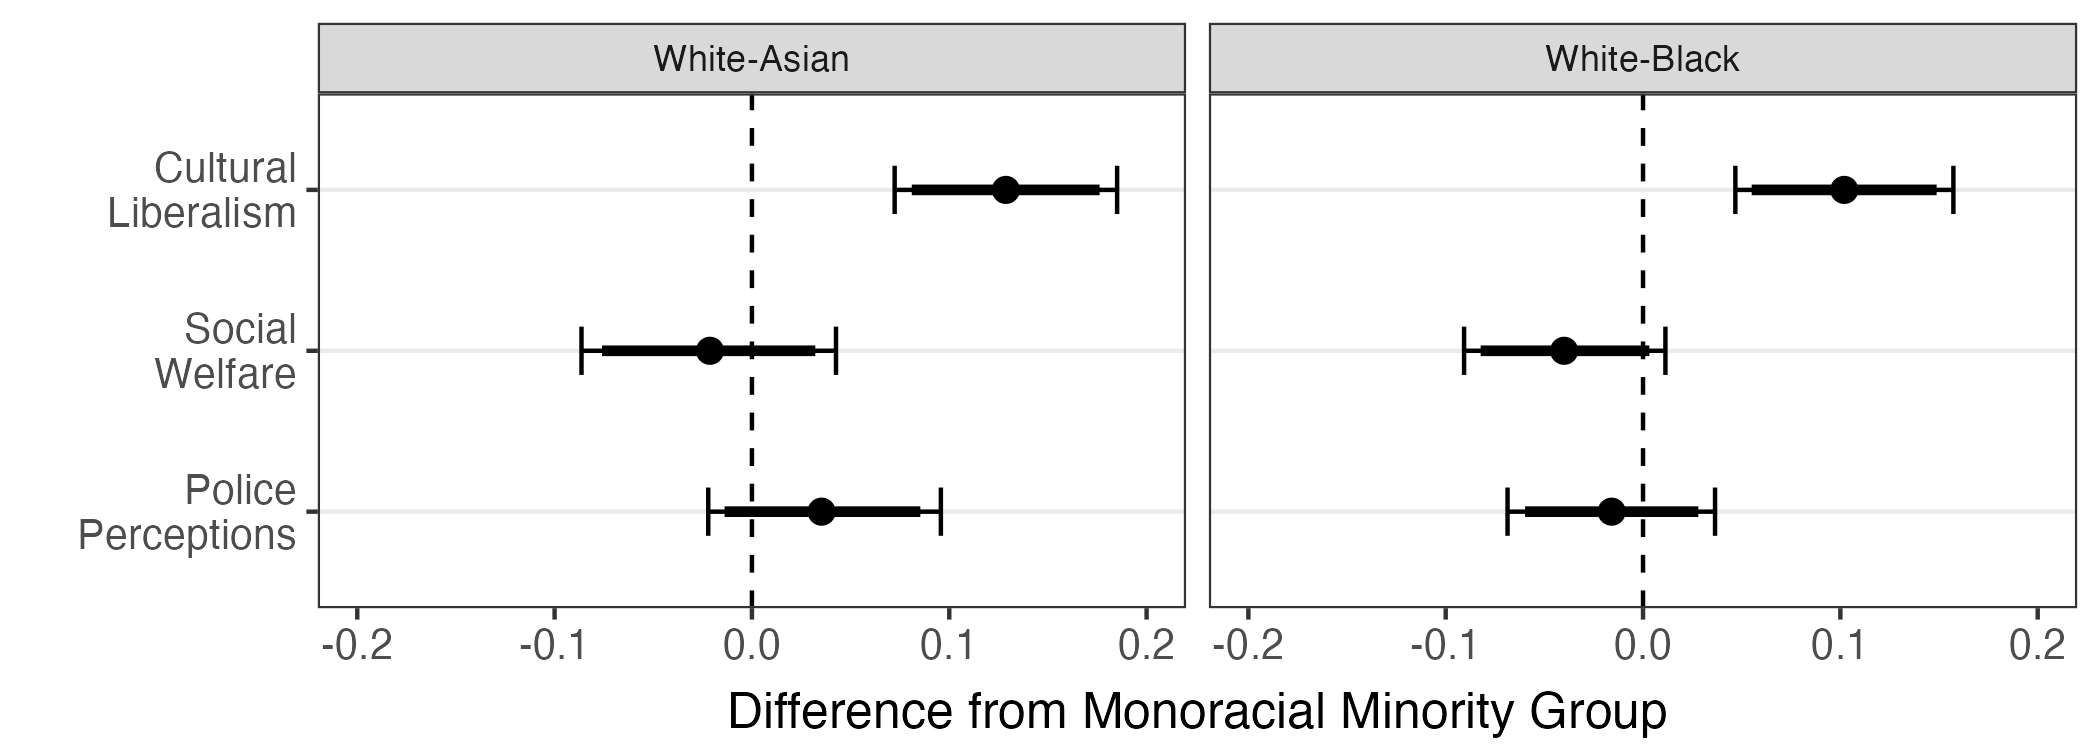
\includegraphics[width=1\textwidth,height=\textheight]{./figures/figure1_prechange.png}

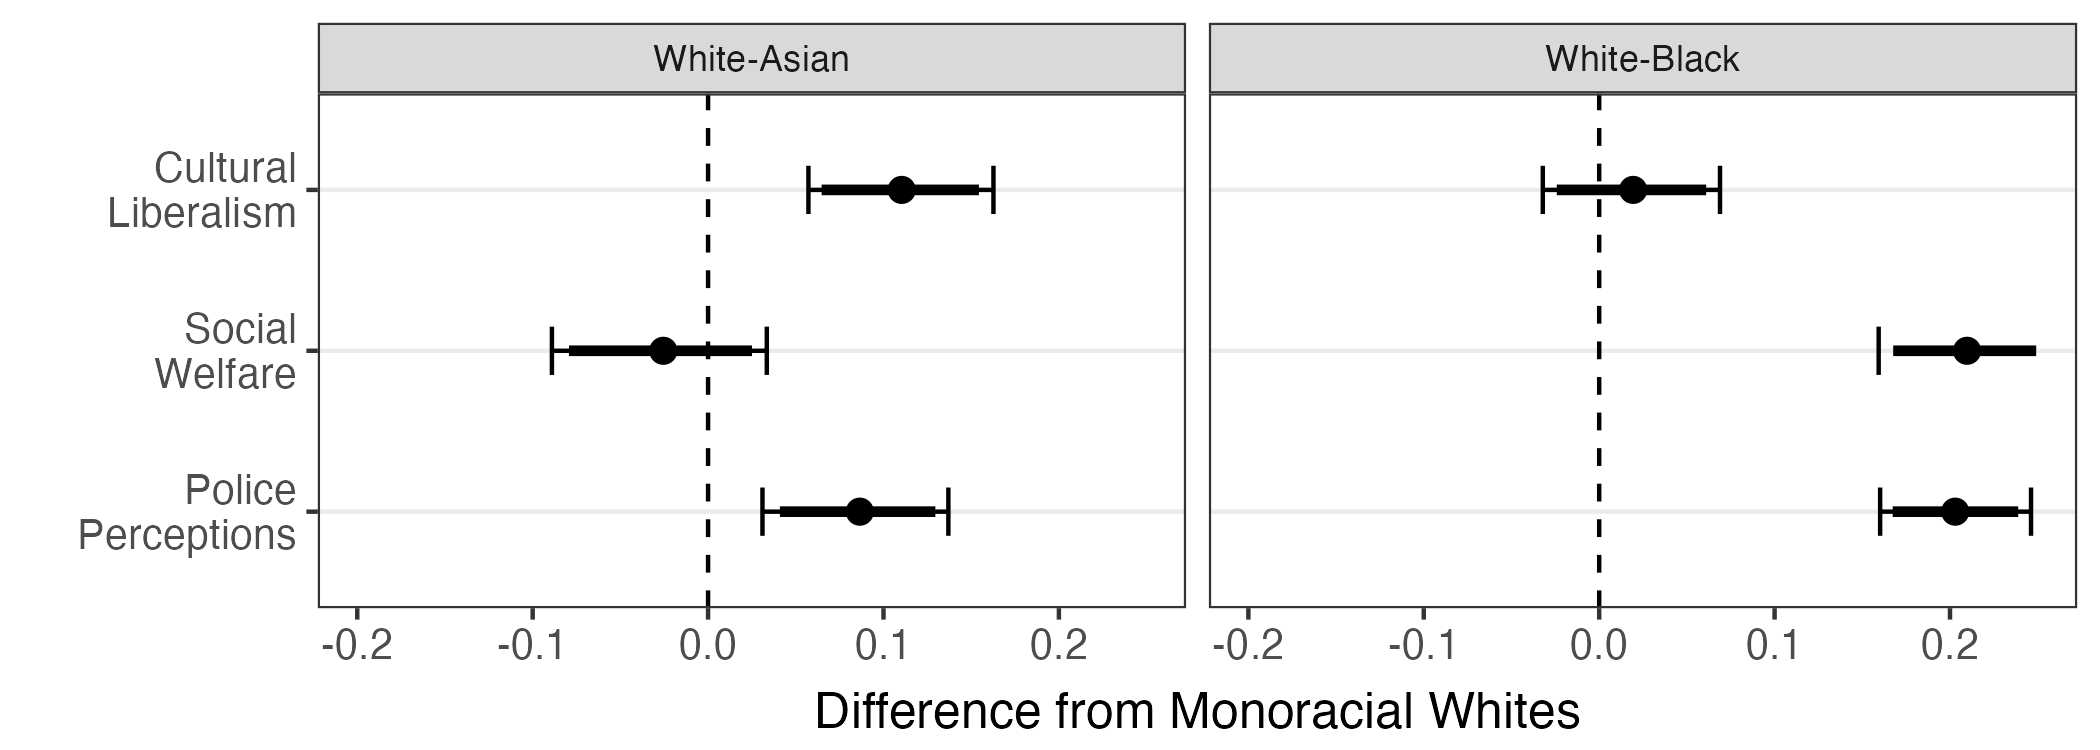
\includegraphics[width=1\textwidth,height=\textheight]{./figures/figure2_prechange.png}

The authors note that they use R version 3.6.2. Issue seems to be the
weights the authors use are non-integer and Zelig uses sample() in that
case which following changes to base R yields different results in 3.6.x
and 3.5.x (see http://docs.zeligproject.org/articles/weights.html).
Prior to R 3.6.x RNGkind(sample.kind = ``Rounding'') was the default
behaviour but after 3.6.0 the sample function's new default behaviour is
RNGkind(sample.kind = ``Rejection'') (see
https://blog.revolutionanalytics.com/2019/05/whats-new-in-r-360.html).

Soemthing about how there are ways to ensure that the estimates are
consistent (changing the weights to integers or setting the RNGkind to
be backwards compatible) but documenting the correct version of R used
in the analysis is probably the easiest way. Segue into\ldots{}

\newpage

\hypertarget{discussion}{%
\section{Discussion}\label{discussion}}

\hypertarget{the-problem-is-the-seed}{%
\subsection{The problem is the seed?}\label{the-problem-is-the-seed}}

The table below shows the quantiles of the means obtained from 100 runs
with 100 different random seeds on R version 3.5 for the \texttt{m2m}
models. We should check where the coefficients from the original paper
fall in that distribution, and see if coefficients should vary so much
simply from changing the seed?

\begin{Shaded}
\begin{Highlighting}[]
\NormalTok{simulations\_m2m\_paths }\OtherTok{\textless{}{-}} \FunctionTok{list.files}\NormalTok{(}\StringTok{"../docker/version\_3.x\_many\_seeds/original/shared\_folder/"}\NormalTok{, }\AttributeTok{pattern =} \StringTok{"m2m.*3\_5.*}\SpecialCharTok{\textbackslash{}\textbackslash{}}\StringTok{d\{1,\}.rds"}\NormalTok{, }\AttributeTok{full.names =} \ConstantTok{TRUE}\NormalTok{)}

\NormalTok{simulations\_m2m }\OtherTok{\textless{}{-}} \FunctionTok{tibble}\NormalTok{(}\AttributeTok{paths =}\NormalTok{ simulations\_m2m\_paths) }\SpecialCharTok{\%\textgreater{}\%}
  \FunctionTok{mutate}\NormalTok{(}\AttributeTok{datasets =} \FunctionTok{map}\NormalTok{(paths, readRDS),}
         \AttributeTok{paths =} \FunctionTok{str\_extract}\NormalTok{(paths, }\StringTok{"}\SpecialCharTok{\textbackslash{}\textbackslash{}}\StringTok{d\{1,\}.rds"}\NormalTok{)) }\SpecialCharTok{\%\textgreater{}\%}
  \FunctionTok{unnest}\NormalTok{(}\AttributeTok{cols =} \FunctionTok{c}\NormalTok{(datasets))}

\NormalTok{simulations\_m2m }\SpecialCharTok{\%\textgreater{}\%}
  \FunctionTok{group\_by}\NormalTok{(race, model) }\SpecialCharTok{\%\textgreater{}\%}
  \FunctionTok{summarise}\NormalTok{(}
    \AttributeTok{q\_005\_mean =} \FunctionTok{quantile}\NormalTok{(mean, }\AttributeTok{probs =} \FloatTok{0.05}\NormalTok{),}
    \AttributeTok{q\_20\_mean =} \FunctionTok{quantile}\NormalTok{(mean, }\AttributeTok{probs =} \FloatTok{0.2}\NormalTok{),}
    \AttributeTok{q\_40\_mean =} \FunctionTok{quantile}\NormalTok{(mean, }\AttributeTok{probs =} \FloatTok{0.4}\NormalTok{),}
    \AttributeTok{q\_50\_mean =} \FunctionTok{quantile}\NormalTok{(mean, }\AttributeTok{probs =} \FloatTok{0.5}\NormalTok{),}
    \AttributeTok{q\_60\_mean =} \FunctionTok{quantile}\NormalTok{(mean, }\AttributeTok{probs =} \FloatTok{0.6}\NormalTok{),}
    \AttributeTok{q\_80\_mean =} \FunctionTok{quantile}\NormalTok{(mean, }\AttributeTok{probs =} \FloatTok{0.8}\NormalTok{),}
    \AttributeTok{q\_95\_mean =} \FunctionTok{quantile}\NormalTok{(mean, }\AttributeTok{probs =} \FloatTok{0.95}\NormalTok{)}
\NormalTok{  ) }\SpecialCharTok{\%\textgreater{}\%}
  \FunctionTok{flextable}\NormalTok{()}
\end{Highlighting}
\end{Shaded}

\begin{verbatim}
`summarise()` has grouped output by 'race'. You can override using the
`.groups` argument.
\end{verbatim}

\global\setlength{\Oldarrayrulewidth}{\arrayrulewidth}

\global\setlength{\Oldtabcolsep}{\tabcolsep}

\setlength{\tabcolsep}{0pt}

\renewcommand*{\arraystretch}{1.5}



\providecommand{\ascline}[3]{\noalign{\global\arrayrulewidth #1}\arrayrulecolor[HTML]{#2}\cline{#3}}

\begin{longtable*}[c]{|p{0.75in}|p{0.75in}|p{0.75in}|p{0.75in}|p{0.75in}|p{0.75in}|p{0.75in}|p{0.75in}|p{0.75in}}



\ascline{1.5pt}{666666}{1-9}

\multicolumn{1}{>{\raggedright}m{\dimexpr 0.75in+0\tabcolsep}}{\textcolor[HTML]{000000}{\fontsize{11}{11}\selectfont{race}}} & \multicolumn{1}{>{\raggedright}m{\dimexpr 0.75in+0\tabcolsep}}{\textcolor[HTML]{000000}{\fontsize{11}{11}\selectfont{model}}} & \multicolumn{1}{>{\raggedleft}m{\dimexpr 0.75in+0\tabcolsep}}{\textcolor[HTML]{000000}{\fontsize{11}{11}\selectfont{q\_005\_mean}}} & \multicolumn{1}{>{\raggedleft}m{\dimexpr 0.75in+0\tabcolsep}}{\textcolor[HTML]{000000}{\fontsize{11}{11}\selectfont{q\_20\_mean}}} & \multicolumn{1}{>{\raggedleft}m{\dimexpr 0.75in+0\tabcolsep}}{\textcolor[HTML]{000000}{\fontsize{11}{11}\selectfont{q\_40\_mean}}} & \multicolumn{1}{>{\raggedleft}m{\dimexpr 0.75in+0\tabcolsep}}{\textcolor[HTML]{000000}{\fontsize{11}{11}\selectfont{q\_50\_mean}}} & \multicolumn{1}{>{\raggedleft}m{\dimexpr 0.75in+0\tabcolsep}}{\textcolor[HTML]{000000}{\fontsize{11}{11}\selectfont{q\_60\_mean}}} & \multicolumn{1}{>{\raggedleft}m{\dimexpr 0.75in+0\tabcolsep}}{\textcolor[HTML]{000000}{\fontsize{11}{11}\selectfont{q\_80\_mean}}} & \multicolumn{1}{>{\raggedleft}m{\dimexpr 0.75in+0\tabcolsep}}{\textcolor[HTML]{000000}{\fontsize{11}{11}\selectfont{q\_95\_mean}}} \\

\ascline{1.5pt}{666666}{1-9}\endhead



\multicolumn{1}{>{\raggedright}m{\dimexpr 0.75in+0\tabcolsep}}{\textcolor[HTML]{000000}{\fontsize{11}{11}\selectfont{White-Asian}}} & \multicolumn{1}{>{\raggedright}m{\dimexpr 0.75in+0\tabcolsep}}{\textcolor[HTML]{000000}{\fontsize{11}{11}\selectfont{Police}}\textcolor[HTML]{000000}{\fontsize{11}{11}\selectfont{\linebreak }}\textcolor[HTML]{000000}{\fontsize{11}{11}\selectfont{Perceptions}}} & \multicolumn{1}{>{\raggedleft}m{\dimexpr 0.75in+0\tabcolsep}}{\textcolor[HTML]{000000}{\fontsize{11}{11}\selectfont{-0.01526542}}} & \multicolumn{1}{>{\raggedleft}m{\dimexpr 0.75in+0\tabcolsep}}{\textcolor[HTML]{000000}{\fontsize{11}{11}\selectfont{-0.001102816}}} & \multicolumn{1}{>{\raggedleft}m{\dimexpr 0.75in+0\tabcolsep}}{\textcolor[HTML]{000000}{\fontsize{11}{11}\selectfont{0.01759581}}} & \multicolumn{1}{>{\raggedleft}m{\dimexpr 0.75in+0\tabcolsep}}{\textcolor[HTML]{000000}{\fontsize{11}{11}\selectfont{0.02586489}}} & \multicolumn{1}{>{\raggedleft}m{\dimexpr 0.75in+0\tabcolsep}}{\textcolor[HTML]{000000}{\fontsize{11}{11}\selectfont{0.03099894}}} & \multicolumn{1}{>{\raggedleft}m{\dimexpr 0.75in+0\tabcolsep}}{\textcolor[HTML]{000000}{\fontsize{11}{11}\selectfont{0.04413257}}} & \multicolumn{1}{>{\raggedleft}m{\dimexpr 0.75in+0\tabcolsep}}{\textcolor[HTML]{000000}{\fontsize{11}{11}\selectfont{0.065472091}}} \\





\multicolumn{1}{>{\raggedright}m{\dimexpr 0.75in+0\tabcolsep}}{\textcolor[HTML]{000000}{\fontsize{11}{11}\selectfont{White-Asian}}} & \multicolumn{1}{>{\raggedright}m{\dimexpr 0.75in+0\tabcolsep}}{\textcolor[HTML]{000000}{\fontsize{11}{11}\selectfont{Social}}\textcolor[HTML]{000000}{\fontsize{11}{11}\selectfont{\linebreak }}\textcolor[HTML]{000000}{\fontsize{11}{11}\selectfont{Welfare}}} & \multicolumn{1}{>{\raggedleft}m{\dimexpr 0.75in+0\tabcolsep}}{\textcolor[HTML]{000000}{\fontsize{11}{11}\selectfont{-0.02072013}}} & \multicolumn{1}{>{\raggedleft}m{\dimexpr 0.75in+0\tabcolsep}}{\textcolor[HTML]{000000}{\fontsize{11}{11}\selectfont{0.006649473}}} & \multicolumn{1}{>{\raggedleft}m{\dimexpr 0.75in+0\tabcolsep}}{\textcolor[HTML]{000000}{\fontsize{11}{11}\selectfont{0.01944720}}} & \multicolumn{1}{>{\raggedleft}m{\dimexpr 0.75in+0\tabcolsep}}{\textcolor[HTML]{000000}{\fontsize{11}{11}\selectfont{0.03262676}}} & \multicolumn{1}{>{\raggedleft}m{\dimexpr 0.75in+0\tabcolsep}}{\textcolor[HTML]{000000}{\fontsize{11}{11}\selectfont{0.03905241}}} & \multicolumn{1}{>{\raggedleft}m{\dimexpr 0.75in+0\tabcolsep}}{\textcolor[HTML]{000000}{\fontsize{11}{11}\selectfont{0.05812758}}} & \multicolumn{1}{>{\raggedleft}m{\dimexpr 0.75in+0\tabcolsep}}{\textcolor[HTML]{000000}{\fontsize{11}{11}\selectfont{0.079513026}}} \\





\multicolumn{1}{>{\raggedright}m{\dimexpr 0.75in+0\tabcolsep}}{\textcolor[HTML]{000000}{\fontsize{11}{11}\selectfont{White-Asian}}} & \multicolumn{1}{>{\raggedright}m{\dimexpr 0.75in+0\tabcolsep}}{\textcolor[HTML]{000000}{\fontsize{11}{11}\selectfont{Cultural}}\textcolor[HTML]{000000}{\fontsize{11}{11}\selectfont{\linebreak }}\textcolor[HTML]{000000}{\fontsize{11}{11}\selectfont{Liberalism}}} & \multicolumn{1}{>{\raggedleft}m{\dimexpr 0.75in+0\tabcolsep}}{\textcolor[HTML]{000000}{\fontsize{11}{11}\selectfont{0.07802019}}} & \multicolumn{1}{>{\raggedleft}m{\dimexpr 0.75in+0\tabcolsep}}{\textcolor[HTML]{000000}{\fontsize{11}{11}\selectfont{0.098207422}}} & \multicolumn{1}{>{\raggedleft}m{\dimexpr 0.75in+0\tabcolsep}}{\textcolor[HTML]{000000}{\fontsize{11}{11}\selectfont{0.11239090}}} & \multicolumn{1}{>{\raggedleft}m{\dimexpr 0.75in+0\tabcolsep}}{\textcolor[HTML]{000000}{\fontsize{11}{11}\selectfont{0.12270775}}} & \multicolumn{1}{>{\raggedleft}m{\dimexpr 0.75in+0\tabcolsep}}{\textcolor[HTML]{000000}{\fontsize{11}{11}\selectfont{0.13180765}}} & \multicolumn{1}{>{\raggedleft}m{\dimexpr 0.75in+0\tabcolsep}}{\textcolor[HTML]{000000}{\fontsize{11}{11}\selectfont{0.14661806}}} & \multicolumn{1}{>{\raggedleft}m{\dimexpr 0.75in+0\tabcolsep}}{\textcolor[HTML]{000000}{\fontsize{11}{11}\selectfont{0.169542042}}} \\





\multicolumn{1}{>{\raggedright}m{\dimexpr 0.75in+0\tabcolsep}}{\textcolor[HTML]{000000}{\fontsize{11}{11}\selectfont{White-Black}}} & \multicolumn{1}{>{\raggedright}m{\dimexpr 0.75in+0\tabcolsep}}{\textcolor[HTML]{000000}{\fontsize{11}{11}\selectfont{Police}}\textcolor[HTML]{000000}{\fontsize{11}{11}\selectfont{\linebreak }}\textcolor[HTML]{000000}{\fontsize{11}{11}\selectfont{Perceptions}}} & \multicolumn{1}{>{\raggedleft}m{\dimexpr 0.75in+0\tabcolsep}}{\textcolor[HTML]{000000}{\fontsize{11}{11}\selectfont{-0.02331918}}} & \multicolumn{1}{>{\raggedleft}m{\dimexpr 0.75in+0\tabcolsep}}{\textcolor[HTML]{000000}{\fontsize{11}{11}\selectfont{-0.001568411}}} & \multicolumn{1}{>{\raggedleft}m{\dimexpr 0.75in+0\tabcolsep}}{\textcolor[HTML]{000000}{\fontsize{11}{11}\selectfont{0.01533537}}} & \multicolumn{1}{>{\raggedleft}m{\dimexpr 0.75in+0\tabcolsep}}{\textcolor[HTML]{000000}{\fontsize{11}{11}\selectfont{0.02181459}}} & \multicolumn{1}{>{\raggedleft}m{\dimexpr 0.75in+0\tabcolsep}}{\textcolor[HTML]{000000}{\fontsize{11}{11}\selectfont{0.02680799}}} & \multicolumn{1}{>{\raggedleft}m{\dimexpr 0.75in+0\tabcolsep}}{\textcolor[HTML]{000000}{\fontsize{11}{11}\selectfont{0.04384726}}} & \multicolumn{1}{>{\raggedleft}m{\dimexpr 0.75in+0\tabcolsep}}{\textcolor[HTML]{000000}{\fontsize{11}{11}\selectfont{0.067172559}}} \\





\multicolumn{1}{>{\raggedright}m{\dimexpr 0.75in+0\tabcolsep}}{\textcolor[HTML]{000000}{\fontsize{11}{11}\selectfont{White-Black}}} & \multicolumn{1}{>{\raggedright}m{\dimexpr 0.75in+0\tabcolsep}}{\textcolor[HTML]{000000}{\fontsize{11}{11}\selectfont{Social}}\textcolor[HTML]{000000}{\fontsize{11}{11}\selectfont{\linebreak }}\textcolor[HTML]{000000}{\fontsize{11}{11}\selectfont{Welfare}}} & \multicolumn{1}{>{\raggedleft}m{\dimexpr 0.75in+0\tabcolsep}}{\textcolor[HTML]{000000}{\fontsize{11}{11}\selectfont{-0.08351311}}} & \multicolumn{1}{>{\raggedleft}m{\dimexpr 0.75in+0\tabcolsep}}{\textcolor[HTML]{000000}{\fontsize{11}{11}\selectfont{-0.062048288}}} & \multicolumn{1}{>{\raggedleft}m{\dimexpr 0.75in+0\tabcolsep}}{\textcolor[HTML]{000000}{\fontsize{11}{11}\selectfont{-0.04489936}}} & \multicolumn{1}{>{\raggedleft}m{\dimexpr 0.75in+0\tabcolsep}}{\textcolor[HTML]{000000}{\fontsize{11}{11}\selectfont{-0.04136138}}} & \multicolumn{1}{>{\raggedleft}m{\dimexpr 0.75in+0\tabcolsep}}{\textcolor[HTML]{000000}{\fontsize{11}{11}\selectfont{-0.03611174}}} & \multicolumn{1}{>{\raggedleft}m{\dimexpr 0.75in+0\tabcolsep}}{\textcolor[HTML]{000000}{\fontsize{11}{11}\selectfont{-0.02119538}}} & \multicolumn{1}{>{\raggedleft}m{\dimexpr 0.75in+0\tabcolsep}}{\textcolor[HTML]{000000}{\fontsize{11}{11}\selectfont{-0.001704422}}} \\





\multicolumn{1}{>{\raggedright}m{\dimexpr 0.75in+0\tabcolsep}}{\textcolor[HTML]{000000}{\fontsize{11}{11}\selectfont{White-Black}}} & \multicolumn{1}{>{\raggedright}m{\dimexpr 0.75in+0\tabcolsep}}{\textcolor[HTML]{000000}{\fontsize{11}{11}\selectfont{Cultural}}\textcolor[HTML]{000000}{\fontsize{11}{11}\selectfont{\linebreak }}\textcolor[HTML]{000000}{\fontsize{11}{11}\selectfont{Liberalism}}} & \multicolumn{1}{>{\raggedleft}m{\dimexpr 0.75in+0\tabcolsep}}{\textcolor[HTML]{000000}{\fontsize{11}{11}\selectfont{0.03562363}}} & \multicolumn{1}{>{\raggedleft}m{\dimexpr 0.75in+0\tabcolsep}}{\textcolor[HTML]{000000}{\fontsize{11}{11}\selectfont{0.060164495}}} & \multicolumn{1}{>{\raggedleft}m{\dimexpr 0.75in+0\tabcolsep}}{\textcolor[HTML]{000000}{\fontsize{11}{11}\selectfont{0.07291920}}} & \multicolumn{1}{>{\raggedleft}m{\dimexpr 0.75in+0\tabcolsep}}{\textcolor[HTML]{000000}{\fontsize{11}{11}\selectfont{0.07738611}}} & \multicolumn{1}{>{\raggedleft}m{\dimexpr 0.75in+0\tabcolsep}}{\textcolor[HTML]{000000}{\fontsize{11}{11}\selectfont{0.08234863}}} & \multicolumn{1}{>{\raggedleft}m{\dimexpr 0.75in+0\tabcolsep}}{\textcolor[HTML]{000000}{\fontsize{11}{11}\selectfont{0.10201330}}} & \multicolumn{1}{>{\raggedleft}m{\dimexpr 0.75in+0\tabcolsep}}{\textcolor[HTML]{000000}{\fontsize{11}{11}\selectfont{0.119382119}}} \\

\ascline{1.5pt}{666666}{1-9}



\end{longtable*}



\arrayrulecolor[HTML]{000000}

\global\setlength{\arrayrulewidth}{\Oldarrayrulewidth}

\global\setlength{\tabcolsep}{\Oldtabcolsep}

\renewcommand*{\arraystretch}{1}

The table below shows the quantiles of the means obtained from 100 runs
with 100 different random seeds on R version 3.5 for the \texttt{m2w}
models:

\begin{Shaded}
\begin{Highlighting}[]
\NormalTok{simulations\_m2w\_paths }\OtherTok{\textless{}{-}} \FunctionTok{list.files}\NormalTok{(}\StringTok{"../docker/version\_3.x\_many\_seeds/original/shared\_folder/"}\NormalTok{, }\AttributeTok{pattern =} \StringTok{"m2w.*3\_5.*}\SpecialCharTok{\textbackslash{}\textbackslash{}}\StringTok{d\{1,\}.rds"}\NormalTok{, }\AttributeTok{full.names =} \ConstantTok{TRUE}\NormalTok{)}

\NormalTok{simulations\_m2w }\OtherTok{\textless{}{-}} \FunctionTok{tibble}\NormalTok{(}\AttributeTok{paths =}\NormalTok{ simulations\_m2w\_paths) }\SpecialCharTok{\%\textgreater{}\%}
  \FunctionTok{mutate}\NormalTok{(}\AttributeTok{datasets =} \FunctionTok{map}\NormalTok{(paths, readRDS),}
         \AttributeTok{paths =} \FunctionTok{str\_extract}\NormalTok{(paths, }\StringTok{"}\SpecialCharTok{\textbackslash{}\textbackslash{}}\StringTok{d\{1,\}.rds"}\NormalTok{)) }\SpecialCharTok{\%\textgreater{}\%}
  \FunctionTok{unnest}\NormalTok{(}\AttributeTok{cols =} \FunctionTok{c}\NormalTok{(datasets))}

\NormalTok{simulations\_m2w }\SpecialCharTok{\%\textgreater{}\%}
  \FunctionTok{group\_by}\NormalTok{(race, model) }\SpecialCharTok{\%\textgreater{}\%}
  \FunctionTok{summarise}\NormalTok{(}
    \AttributeTok{q\_005\_mean =} \FunctionTok{quantile}\NormalTok{(mean, }\AttributeTok{probs =} \FloatTok{0.05}\NormalTok{),}
    \AttributeTok{q\_20\_mean =} \FunctionTok{quantile}\NormalTok{(mean, }\AttributeTok{probs =} \FloatTok{0.2}\NormalTok{),}
    \AttributeTok{q\_40\_mean =} \FunctionTok{quantile}\NormalTok{(mean, }\AttributeTok{probs =} \FloatTok{0.4}\NormalTok{),}
    \AttributeTok{q\_50\_mean =} \FunctionTok{quantile}\NormalTok{(mean, }\AttributeTok{probs =} \FloatTok{0.5}\NormalTok{),}
    \AttributeTok{q\_60\_mean =} \FunctionTok{quantile}\NormalTok{(mean, }\AttributeTok{probs =} \FloatTok{0.6}\NormalTok{),}
    \AttributeTok{q\_80\_mean =} \FunctionTok{quantile}\NormalTok{(mean, }\AttributeTok{probs =} \FloatTok{0.8}\NormalTok{),}
    \AttributeTok{q\_95\_mean =} \FunctionTok{quantile}\NormalTok{(mean, }\AttributeTok{probs =} \FloatTok{0.95}\NormalTok{)}
\NormalTok{  ) }\SpecialCharTok{\%\textgreater{}\%}
  \FunctionTok{flextable}\NormalTok{()}
\end{Highlighting}
\end{Shaded}

\begin{verbatim}
`summarise()` has grouped output by 'race'. You can override using the
`.groups` argument.
\end{verbatim}

\global\setlength{\Oldarrayrulewidth}{\arrayrulewidth}

\global\setlength{\Oldtabcolsep}{\tabcolsep}

\setlength{\tabcolsep}{0pt}

\renewcommand*{\arraystretch}{1.5}



\providecommand{\ascline}[3]{\noalign{\global\arrayrulewidth #1}\arrayrulecolor[HTML]{#2}\cline{#3}}

\begin{longtable*}[c]{|p{0.75in}|p{0.75in}|p{0.75in}|p{0.75in}|p{0.75in}|p{0.75in}|p{0.75in}|p{0.75in}|p{0.75in}}



\ascline{1.5pt}{666666}{1-9}

\multicolumn{1}{>{\raggedright}m{\dimexpr 0.75in+0\tabcolsep}}{\textcolor[HTML]{000000}{\fontsize{11}{11}\selectfont{race}}} & \multicolumn{1}{>{\raggedright}m{\dimexpr 0.75in+0\tabcolsep}}{\textcolor[HTML]{000000}{\fontsize{11}{11}\selectfont{model}}} & \multicolumn{1}{>{\raggedleft}m{\dimexpr 0.75in+0\tabcolsep}}{\textcolor[HTML]{000000}{\fontsize{11}{11}\selectfont{q\_005\_mean}}} & \multicolumn{1}{>{\raggedleft}m{\dimexpr 0.75in+0\tabcolsep}}{\textcolor[HTML]{000000}{\fontsize{11}{11}\selectfont{q\_20\_mean}}} & \multicolumn{1}{>{\raggedleft}m{\dimexpr 0.75in+0\tabcolsep}}{\textcolor[HTML]{000000}{\fontsize{11}{11}\selectfont{q\_40\_mean}}} & \multicolumn{1}{>{\raggedleft}m{\dimexpr 0.75in+0\tabcolsep}}{\textcolor[HTML]{000000}{\fontsize{11}{11}\selectfont{q\_50\_mean}}} & \multicolumn{1}{>{\raggedleft}m{\dimexpr 0.75in+0\tabcolsep}}{\textcolor[HTML]{000000}{\fontsize{11}{11}\selectfont{q\_60\_mean}}} & \multicolumn{1}{>{\raggedleft}m{\dimexpr 0.75in+0\tabcolsep}}{\textcolor[HTML]{000000}{\fontsize{11}{11}\selectfont{q\_80\_mean}}} & \multicolumn{1}{>{\raggedleft}m{\dimexpr 0.75in+0\tabcolsep}}{\textcolor[HTML]{000000}{\fontsize{11}{11}\selectfont{q\_95\_mean}}} \\

\ascline{1.5pt}{666666}{1-9}\endhead



\multicolumn{1}{>{\raggedright}m{\dimexpr 0.75in+0\tabcolsep}}{\textcolor[HTML]{000000}{\fontsize{11}{11}\selectfont{White-Asian}}} & \multicolumn{1}{>{\raggedright}m{\dimexpr 0.75in+0\tabcolsep}}{\textcolor[HTML]{000000}{\fontsize{11}{11}\selectfont{Police}}\textcolor[HTML]{000000}{\fontsize{11}{11}\selectfont{\linebreak }}\textcolor[HTML]{000000}{\fontsize{11}{11}\selectfont{Perceptions}}} & \multicolumn{1}{>{\raggedleft}m{\dimexpr 0.75in+0\tabcolsep}}{\textcolor[HTML]{000000}{\fontsize{11}{11}\selectfont{0.046735795}}} & \multicolumn{1}{>{\raggedleft}m{\dimexpr 0.75in+0\tabcolsep}}{\textcolor[HTML]{000000}{\fontsize{11}{11}\selectfont{0.067470058}}} & \multicolumn{1}{>{\raggedleft}m{\dimexpr 0.75in+0\tabcolsep}}{\textcolor[HTML]{000000}{\fontsize{11}{11}\selectfont{0.08117265}}} & \multicolumn{1}{>{\raggedleft}m{\dimexpr 0.75in+0\tabcolsep}}{\textcolor[HTML]{000000}{\fontsize{11}{11}\selectfont{0.09007913}}} & \multicolumn{1}{>{\raggedleft}m{\dimexpr 0.75in+0\tabcolsep}}{\textcolor[HTML]{000000}{\fontsize{11}{11}\selectfont{0.09895873}}} & \multicolumn{1}{>{\raggedleft}m{\dimexpr 0.75in+0\tabcolsep}}{\textcolor[HTML]{000000}{\fontsize{11}{11}\selectfont{0.11565896}}} & \multicolumn{1}{>{\raggedleft}m{\dimexpr 0.75in+0\tabcolsep}}{\textcolor[HTML]{000000}{\fontsize{11}{11}\selectfont{0.13773174}}} \\





\multicolumn{1}{>{\raggedright}m{\dimexpr 0.75in+0\tabcolsep}}{\textcolor[HTML]{000000}{\fontsize{11}{11}\selectfont{White-Asian}}} & \multicolumn{1}{>{\raggedright}m{\dimexpr 0.75in+0\tabcolsep}}{\textcolor[HTML]{000000}{\fontsize{11}{11}\selectfont{Social}}\textcolor[HTML]{000000}{\fontsize{11}{11}\selectfont{\linebreak }}\textcolor[HTML]{000000}{\fontsize{11}{11}\selectfont{Welfare}}} & \multicolumn{1}{>{\raggedleft}m{\dimexpr 0.75in+0\tabcolsep}}{\textcolor[HTML]{000000}{\fontsize{11}{11}\selectfont{-0.004927122}}} & \multicolumn{1}{>{\raggedleft}m{\dimexpr 0.75in+0\tabcolsep}}{\textcolor[HTML]{000000}{\fontsize{11}{11}\selectfont{0.020943227}}} & \multicolumn{1}{>{\raggedleft}m{\dimexpr 0.75in+0\tabcolsep}}{\textcolor[HTML]{000000}{\fontsize{11}{11}\selectfont{0.03311780}}} & \multicolumn{1}{>{\raggedleft}m{\dimexpr 0.75in+0\tabcolsep}}{\textcolor[HTML]{000000}{\fontsize{11}{11}\selectfont{0.05020756}}} & \multicolumn{1}{>{\raggedleft}m{\dimexpr 0.75in+0\tabcolsep}}{\textcolor[HTML]{000000}{\fontsize{11}{11}\selectfont{0.05851728}}} & \multicolumn{1}{>{\raggedleft}m{\dimexpr 0.75in+0\tabcolsep}}{\textcolor[HTML]{000000}{\fontsize{11}{11}\selectfont{0.07343161}}} & \multicolumn{1}{>{\raggedleft}m{\dimexpr 0.75in+0\tabcolsep}}{\textcolor[HTML]{000000}{\fontsize{11}{11}\selectfont{0.10264449}}} \\





\multicolumn{1}{>{\raggedright}m{\dimexpr 0.75in+0\tabcolsep}}{\textcolor[HTML]{000000}{\fontsize{11}{11}\selectfont{White-Asian}}} & \multicolumn{1}{>{\raggedright}m{\dimexpr 0.75in+0\tabcolsep}}{\textcolor[HTML]{000000}{\fontsize{11}{11}\selectfont{Cultural}}\textcolor[HTML]{000000}{\fontsize{11}{11}\selectfont{\linebreak }}\textcolor[HTML]{000000}{\fontsize{11}{11}\selectfont{Liberalism}}} & \multicolumn{1}{>{\raggedleft}m{\dimexpr 0.75in+0\tabcolsep}}{\textcolor[HTML]{000000}{\fontsize{11}{11}\selectfont{0.046796515}}} & \multicolumn{1}{>{\raggedleft}m{\dimexpr 0.75in+0\tabcolsep}}{\textcolor[HTML]{000000}{\fontsize{11}{11}\selectfont{0.062335404}}} & \multicolumn{1}{>{\raggedleft}m{\dimexpr 0.75in+0\tabcolsep}}{\textcolor[HTML]{000000}{\fontsize{11}{11}\selectfont{0.08756450}}} & \multicolumn{1}{>{\raggedleft}m{\dimexpr 0.75in+0\tabcolsep}}{\textcolor[HTML]{000000}{\fontsize{11}{11}\selectfont{0.09205009}}} & \multicolumn{1}{>{\raggedleft}m{\dimexpr 0.75in+0\tabcolsep}}{\textcolor[HTML]{000000}{\fontsize{11}{11}\selectfont{0.09816402}}} & \multicolumn{1}{>{\raggedleft}m{\dimexpr 0.75in+0\tabcolsep}}{\textcolor[HTML]{000000}{\fontsize{11}{11}\selectfont{0.11266966}}} & \multicolumn{1}{>{\raggedleft}m{\dimexpr 0.75in+0\tabcolsep}}{\textcolor[HTML]{000000}{\fontsize{11}{11}\selectfont{0.13290792}}} \\





\multicolumn{1}{>{\raggedright}m{\dimexpr 0.75in+0\tabcolsep}}{\textcolor[HTML]{000000}{\fontsize{11}{11}\selectfont{White-Black}}} & \multicolumn{1}{>{\raggedright}m{\dimexpr 0.75in+0\tabcolsep}}{\textcolor[HTML]{000000}{\fontsize{11}{11}\selectfont{Police}}\textcolor[HTML]{000000}{\fontsize{11}{11}\selectfont{\linebreak }}\textcolor[HTML]{000000}{\fontsize{11}{11}\selectfont{Perceptions}}} & \multicolumn{1}{>{\raggedleft}m{\dimexpr 0.75in+0\tabcolsep}}{\textcolor[HTML]{000000}{\fontsize{11}{11}\selectfont{0.169510723}}} & \multicolumn{1}{>{\raggedleft}m{\dimexpr 0.75in+0\tabcolsep}}{\textcolor[HTML]{000000}{\fontsize{11}{11}\selectfont{0.189838189}}} & \multicolumn{1}{>{\raggedleft}m{\dimexpr 0.75in+0\tabcolsep}}{\textcolor[HTML]{000000}{\fontsize{11}{11}\selectfont{0.20124209}}} & \multicolumn{1}{>{\raggedleft}m{\dimexpr 0.75in+0\tabcolsep}}{\textcolor[HTML]{000000}{\fontsize{11}{11}\selectfont{0.20983966}}} & \multicolumn{1}{>{\raggedleft}m{\dimexpr 0.75in+0\tabcolsep}}{\textcolor[HTML]{000000}{\fontsize{11}{11}\selectfont{0.21606705}}} & \multicolumn{1}{>{\raggedleft}m{\dimexpr 0.75in+0\tabcolsep}}{\textcolor[HTML]{000000}{\fontsize{11}{11}\selectfont{0.23216549}}} & \multicolumn{1}{>{\raggedleft}m{\dimexpr 0.75in+0\tabcolsep}}{\textcolor[HTML]{000000}{\fontsize{11}{11}\selectfont{0.26767669}}} \\





\multicolumn{1}{>{\raggedright}m{\dimexpr 0.75in+0\tabcolsep}}{\textcolor[HTML]{000000}{\fontsize{11}{11}\selectfont{White-Black}}} & \multicolumn{1}{>{\raggedright}m{\dimexpr 0.75in+0\tabcolsep}}{\textcolor[HTML]{000000}{\fontsize{11}{11}\selectfont{Social}}\textcolor[HTML]{000000}{\fontsize{11}{11}\selectfont{\linebreak }}\textcolor[HTML]{000000}{\fontsize{11}{11}\selectfont{Welfare}}} & \multicolumn{1}{>{\raggedleft}m{\dimexpr 0.75in+0\tabcolsep}}{\textcolor[HTML]{000000}{\fontsize{11}{11}\selectfont{0.154936922}}} & \multicolumn{1}{>{\raggedleft}m{\dimexpr 0.75in+0\tabcolsep}}{\textcolor[HTML]{000000}{\fontsize{11}{11}\selectfont{0.177350470}}} & \multicolumn{1}{>{\raggedleft}m{\dimexpr 0.75in+0\tabcolsep}}{\textcolor[HTML]{000000}{\fontsize{11}{11}\selectfont{0.19262474}}} & \multicolumn{1}{>{\raggedleft}m{\dimexpr 0.75in+0\tabcolsep}}{\textcolor[HTML]{000000}{\fontsize{11}{11}\selectfont{0.19770454}}} & \multicolumn{1}{>{\raggedleft}m{\dimexpr 0.75in+0\tabcolsep}}{\textcolor[HTML]{000000}{\fontsize{11}{11}\selectfont{0.20252183}}} & \multicolumn{1}{>{\raggedleft}m{\dimexpr 0.75in+0\tabcolsep}}{\textcolor[HTML]{000000}{\fontsize{11}{11}\selectfont{0.22472549}}} & \multicolumn{1}{>{\raggedleft}m{\dimexpr 0.75in+0\tabcolsep}}{\textcolor[HTML]{000000}{\fontsize{11}{11}\selectfont{0.24515122}}} \\





\multicolumn{1}{>{\raggedright}m{\dimexpr 0.75in+0\tabcolsep}}{\textcolor[HTML]{000000}{\fontsize{11}{11}\selectfont{White-Black}}} & \multicolumn{1}{>{\raggedright}m{\dimexpr 0.75in+0\tabcolsep}}{\textcolor[HTML]{000000}{\fontsize{11}{11}\selectfont{Cultural}}\textcolor[HTML]{000000}{\fontsize{11}{11}\selectfont{\linebreak }}\textcolor[HTML]{000000}{\fontsize{11}{11}\selectfont{Liberalism}}} & \multicolumn{1}{>{\raggedleft}m{\dimexpr 0.75in+0\tabcolsep}}{\textcolor[HTML]{000000}{\fontsize{11}{11}\selectfont{-0.009211098}}} & \multicolumn{1}{>{\raggedleft}m{\dimexpr 0.75in+0\tabcolsep}}{\textcolor[HTML]{000000}{\fontsize{11}{11}\selectfont{0.008618765}}} & \multicolumn{1}{>{\raggedleft}m{\dimexpr 0.75in+0\tabcolsep}}{\textcolor[HTML]{000000}{\fontsize{11}{11}\selectfont{0.02023309}}} & \multicolumn{1}{>{\raggedleft}m{\dimexpr 0.75in+0\tabcolsep}}{\textcolor[HTML]{000000}{\fontsize{11}{11}\selectfont{0.02625295}}} & \multicolumn{1}{>{\raggedleft}m{\dimexpr 0.75in+0\tabcolsep}}{\textcolor[HTML]{000000}{\fontsize{11}{11}\selectfont{0.02985881}}} & \multicolumn{1}{>{\raggedleft}m{\dimexpr 0.75in+0\tabcolsep}}{\textcolor[HTML]{000000}{\fontsize{11}{11}\selectfont{0.04424369}}} & \multicolumn{1}{>{\raggedleft}m{\dimexpr 0.75in+0\tabcolsep}}{\textcolor[HTML]{000000}{\fontsize{11}{11}\selectfont{0.06153429}}} \\

\ascline{1.5pt}{666666}{1-9}



\end{longtable*}



\arrayrulecolor[HTML]{000000}

\global\setlength{\arrayrulewidth}{\Oldarrayrulewidth}

\global\setlength{\tabcolsep}{\Oldtabcolsep}

\renewcommand*{\arraystretch}{1}

\hypertarget{rebuilding-the-original-development-environment-using-docker}{%
\subsection{Rebuilding the original development environment using
Docker}\label{rebuilding-the-original-development-environment-using-docker}}

Replicating results from past studies is quite challenging, for many
reasons. This articles focuses on one of these reasons: results cannot
be reproduced because of changes introduced in more recent versions of
the software used for analysis, despite the availability of both data
and replication scripts.

To replicate the results from the original study and to pinpoint the
impact of the change introduced in R 3.6.0, we chose to use Docker.
Docker is a containerization tool which enables one to build so-called
\emph{images}. These images contain a software product alongside its
dependencies and even pieces of a Linux operating system. To use the
software product, customers in turn only need to be able to run Docker
\emph{containers} from the image definition. Containerization tools such
as Docker solved the ``works on my machine'' problem: this problem
arises when software that works well on the development machine of the
developer fails to run successfully on a customer's machine. This
usually happens because the customer's computer does not have the
necessary dependencies to run the software (which are traditionally not
shipped alongside the software product).

A research project can also be seen as a \emph{software product}, and
suffers thus from the same ``works on my machine'' problem as any other
type of software. Containerization tools offer a great opportunity for
reproducibility in research: instead of just sharing a replication
script, authors can now easily share the right version of the software
used to produce these scripts, as well as the right version of the used
libraries by building and sharing a Docker image (or at least provide
the necessary blueprint to enable others to do so, as we will discuss
below). Future researchers looking to replicate the results can now
simple run a container from the provided image (or build an image
themselves if the original authors provided the required blueprints).

Concretely, to build a Docker image, a researcher writes a so-called
\emph{Dockerfile}. Here is an example of a very simple Dockerfile:

\begin{verbatim}
FROM rocker/r-ver:4.3.0

CMD ["R"]
\end{verbatim}

This Dockerfile contains two lines: the first line states which Docker
image we are going to use as a base. Our image will be based on the
`rocker/r-ver:4.3.0' image. The Rocker project is a repository
containing many images that ship different versions of R and packages
pre-installed: so the image called \texttt{r-ver:4.3.0} is an image that
ships R version 4.3.0. The last line states which command should run
when the user runs a container defined from our image, so in this case,
simply the R interactive prompt. Below is an example of a Dockerfile
that runs an analysis script:

\begin{verbatim}
FROM rocker/r-ver:4.3.0

RUN R -e "install.packages('dplyr')"

RUN mkdir /home/research_project

RUN mkdir /home/research_project/project_output

RUN mkdir /home/research_project/shared_folder

COPY analyse_data.R /home/research_project/analyse_data.R

RUN cd /home/research_project && R -e "source('analyse_data.R')"

CMD mv /home/research_project/project_output/* /home/research_project/shared_folder/
\end{verbatim}

This Dockerfile starts off from the same base image, an image that ships
R version 4.3.0, than it install the \texttt{\{dplyr\}} package, a
popular R package for data manipulation and it creates three
directories:

\begin{itemize}
\tightlist
\item
  \texttt{/home/research\_project}
\item
  \texttt{/home/research\_project/project\_output}
\item
  \texttt{/home/research\_project/shared\_folder}.
\end{itemize}

Then, it copies the \texttt{analyse\_data.R} script, which contains the
actual analysis made for the purposes of the research project, into the
Docker image. The second-to-last line runs the script, and the last line
moves the outputs generated from running the \texttt{analyse\_data.R}
script to a folder called \texttt{shared\_folder}. It is important to
say that \texttt{RUN} statements will be executed as the image gets
built, and \texttt{CMD} statements will be executed as a container runs.
Using this Dockerfile, an image called \texttt{research\_project} can be
built with the following command:

\begin{verbatim}
docker build -t research_project .
\end{verbatim}

This image can then be archived and shared for replication purposes.
Future researchers can then run a container from that image using a
command such as:

\begin{verbatim}
docker run -d -it --rm --name research_project_container \
  -v /host/machine/shared_folder:/home/research_project/shared_folder:rw \
  research_project
\end{verbatim}

The container, called \texttt{research\_project\_container} will execute
the \texttt{CMD} statement from the Dockerfile, in other words, move the
outputs to the \texttt{shared\_folder}. This folder is like a door
between the machine that runs the container and the container: by doing
this, the outputs generated within the container can now be accessed
from the host's computer.

The image built by the process above is immutable: so as long as users
can run it, the outputs produced will be exactly the same as when the
original author ran the original analysis. However, if the image gets
lost, and needs to be rebuilt, the above Dockerfile will not generate
the same image. This is because the Dockerfile, as it is written above,
will download the version of \texttt{\{dplyr\}} that is current at the
time it gets built. So if a user instead builds the image in 5 years,
the version of \texttt{\{dplyr\}} that will get downloaded. The version
of R, however, will forever remain at version 4.3.0.

So to ensure that future researchers will download the right versions of
packages that were originally used for the project, the original
researcher also needs to provide a list of packages and their versions.
This can be quite tedious if done by hand, but thankfully, there are
ways to generate such lists very easily. The \texttt{\{renv\}} package
for the R programming language provides such a function. Once the
project is done, one simply needs to call:

\begin{verbatim}
renv::init()
renv::hydrate()
renv::snapshot()
\end{verbatim}

to generate a file called \texttt{renv.lock}. This file contains the R
version that was used to generate it, the list of packages that were
used for the project, as well as their versions and links to download
them.

\hypertarget{reproducibility-isnt-just-version-and-package-management-using-targets-to-improve-readibility-and-reproducibility}{%
\subsection{Reproducibility isn't just version and package management
--- using \{targets\} to improve readibility and
reproducibility}\label{reproducibility-isnt-just-version-and-package-management-using-targets-to-improve-readibility-and-reproducibility}}

\newpage

\hypertarget{conclusion}{%
\section{Conclusion}\label{conclusion}}

\newpage

\hypertarget{references}{%
\section*{References}\label{references}}
\addcontentsline{toc}{section}{References}

\hypertarget{refs}{}
\begin{CSLReferences}{1}{0}
\leavevmode\vadjust pre{\hypertarget{ref-davenport2022multiracial}{}}%
Davenport, Lauren, Annie Franco, and Shanto Iyengar. 2022.
{``{Multiracial identity and political preferences}.''} \emph{The
Journal of Politics} 84 (1): 620--24.

\leavevmode\vadjust pre{\hypertarget{ref-philip2010report}{}}%
Philip, Glandon. 2010. {``{Report on the American Economic Review Data
Availability Compliance Project}.''} \emph{Unpublished Manuscript}.

\leavevmode\vadjust pre{\hypertarget{ref-simonsohn95GroundhogAddressing2021}{}}%
Simonsohn, Uri. 2021. {``{[}95{]} {Groundhog}: {Addressing The Threat
That R Poses To Reproducible Research}.''} \emph{Data Colada}.
http://datacolada.org/95.

\leavevmode\vadjust pre{\hypertarget{ref-stockemer2018data}{}}%
Stockemer, Daniel, Sebastian Koehler, and Tobias Lentz. 2018. {``{Data
access, transparency, and replication: New insights from the political
behavior literature}.''} \emph{PS: Political Science \& Politics} 51
(4): 799--803.

\end{CSLReferences}



\end{document}
